
\PassOptionsToPackage{x11names}{xcolor}

\documentclass[symmetric]{tufte-handout}

%\geometry{showframe}% for debugging purposes -- displays the margins



\usepackage{amsmath}
\usepackage{mathtools}
\usepackage{amsfonts}
\usepackage{amsthm}


\usepackage{microtype}


% Set up the images/graphics package
\usepackage{graphicx}
\setkeys{Gin}{width=\linewidth,totalheight=\textheight,keepaspectratio}
\graphicspath{{graphics/}}

\title{Lecture Notes -- The Julia Set}
\author{Josh Lipschultz \& Ricky LeVan}
\date{}  % if the \date{} command is left out, the current date will be used

% The following package makes prettier tables.  We're all about the bling!
\usepackage{booktabs}

% The units package provides nice, non-stacked fractions and better spacing
% for units.
\usepackage{units}

% The fancyvrb package lets us customize the formatting of verbatim
% environments.  We use a slightly smaller font.
\usepackage{fancyvrb}
\fvset{fontsize=\normalsize}

% Small sections of multiple columns
\usepackage{multicol}

% Provides paragraphs of dummy text
\usepackage{lipsum}

% These commands are used to pretty-print LaTeX commands
\newcommand{\doccmd}[1]{\texttt{\textbackslash#1}}% command name -- adds backslash automatically
\newcommand{\docopt}[1]{\ensuremath{\langle}\textrm{\textit{#1}}\ensuremath{\rangle}}% optional command argument
\newcommand{\docarg}[1]{\textrm{\textit{#1}}}% (required) command argument
\newenvironment{docspec}{\begin{quote}\noindent}{\end{quote}}% command specification environment
\newcommand{\docenv}[1]{\textsf{#1}}% environment name
\newcommand{\docpkg}[1]{\texttt{#1}}% package name
\newcommand{\doccls}[1]{\texttt{#1}}% document class name
\newcommand{\docclsopt}[1]{\texttt{#1}}% document class option name



\usepackage{tikz}
\usetikzlibrary{decorations.fractals}
\usetikzlibrary{shadings}
\usepackage{rotating}

\usepackage[ruled, vlined]{algorithm2e}



\definecolor{aqua}{RGB}{63,113,113}
\definecolor{lightaqua}{RGB}{184,222,222}



\newtheorem{theorem}{Theorem}
\newtheorem{corollary}{Corollary}
\newtheorem{definition}{Definition}
\newtheorem{rmk}{Remark}


\begin{document}

\maketitle% this prints the handout title, author, and date



\section{Preliminaries}\label{sec:problem-1}

As a quick recap of what we saw last week, recall the following facts.

The \textsl{stable set} of a a complex polynomial $P: \mathbb{C} \rightarrow \mathbb{C}$, denoted $S(P)$, is the complement of $J(C)$.

Another useful definition was that of a \textsl{bounded orbit}. An orbit is bounded if there exists a $K$ such that $|Q_c^{\circ n}(z)| < K$ for all $n$. Otherwise the orbit is \textsl{unbounded}.

The previous group also discussed how the points of $S^1$ were \textsl{supersensitive}. That is, any open ball $B$ around $z \in S^1$ has the property that $\bigcup_{n=0}^\infty Q_0^{\circ n} (B) = \mathbb{C} \setminus \{p\}$ for at most one point $p$.

We also defined the Julia Set $J_c$ as the boundary of the filled Julia set $K_c$. (The filled Julia set is the set of bounded points of $Q_c$.) We could alternatively define $J_c$ as the closure of the set of repelling points of $Q_c$ (in fact, this definition isn't limited to the quadratic map; any polynomial will do, and is denoted $J(P)$ ).

For the quadratic map $Q_0(z) = z^2$ we saw chaotic behavior only on $S^1$ by angle doubling ($\theta \rightarrow 2\theta$). We also saw that $|Q_0(z)| \rightarrow \infty$ for all $|z| > 1$ and $|Q_0(z)| \rightarrow 0$ for all $|z| < 1$.

Finally, we learned that for $Q_{-2}(z) = z^2 - 2$, we have $J_2 = K_2 = [-2, 2]$, so any $z \in \mathbb{C} \ [-2,2] \rightarrow \infty$ as we compose $Q_{-2}(z)$ infinitely many times. 



\section{16.3 -- The Julia Set as a Cantor Set}\label{sec:problem-1}

\marginnote[-2cm]{
\begin{center}
\begin{sideways}
\begin{tikzpicture}[decoration=Cantor set,very thick]
\draw[DeepSkyBlue4] decorate{ (0,0) -- (10,0) };
\draw[DeepSkyBlue4] decorate{ decorate{ (0,-.5) -- (10,-.5) }};
\draw[DeepSkyBlue4] decorate{ decorate{ decorate{ (0,-1) -- (10,-1) }}};
\draw[DeepSkyBlue4] decorate{ decorate{ decorate{ decorate{ (0,-1.5) -- (10,-1.5) }}}};
\draw[DeepSkyBlue4] decorate{ decorate{ decorate{ decorate{ decorate{ (0,-2) -- (10,-2) }}}}};
\end{tikzpicture}
\end{sideways}
\end{center}
}


Our goal for this section of the talk is to discuss and prove parts of
the following theorem.


\begin{theorem}
If $|c|$ is sufficiently large, $\Lambda$, the set of points whose entire forward orbits lie within the circle $|z|=|c|$, is a Cantor set on which $Q_c$ is topologically conjugate to the shift map on two symbols. All points in $\mathbb{C} - \Lambda$ tend to $\infty$ under iteration of $Q_c$. Hence, $J_c=K_c$.
\end{theorem}



\subsection{Points Which Escape}



\begin{theorem} \label{escape} [The Escape Criterion]
Suppose $2 < |c| \le |z|$. Then we have that $|Q_c^n(z)| \rightarrow \infty$ as $n \rightarrow \infty$.

\end{theorem}
\begin{proof}
We use the triangle inequality to get the following estimate:
\begin{equation}
    |Q_c^n(z)| \geq |z|^2 - |c| \geq |z|^2 - |z| = |z|(|z|-1)
\end{equation}
Since $|z| > 2$, we know that $|z|-1>1$, so there exists $\lambda > 0$ such that 
\begin{equation}
    |Q_c^n(z)| \geq (1+\lambda)^n|z|
\end{equation}
Since $|z|$ is fixed and $(1+\lambda)^n$ grows arbitrarily large, $|Q_c^n(z)|$ also grows arbitrarily large, as desired.

\end{proof}




\subsection{Points Which Escape}




\subsection{The Filled Julia Set}

\begin{theorem}
Let $D$ be the closed disk (i.e. $\{z : |z| \le |c|\}$), with $|c|>2$. Then the filled Julia set of $Q_c$ is given by
\begin{align*}
K_c = \bigcap\limits_{n\ge 0} Q_c^{\circ -n} (D)
\end{align*}
where $Q_c^{\circ -n} (D)$ denotes the preimage of $D$ under $Q_c^{\circ n}$
\end{theorem}

\begin{proof}
    Consider the case where
    $z\notin \bigcap_{n\ge 0} Q_c^{\circ -n} (D)$.
    Then there exists some $k\in \mathbb{N}$ such that $z\notin Q_c^{\circ -k} (D)$,
    so we have that $Q_c^{\circ k}(z) \notin D$. 
    Thus by Theorem~\ref{escape}, $z$ escapes to infinity under iteration
    of $Q_c$, so $z\notin K_c$.  

    Otherwise, if $z\in \bigcap_{n\ge 0} Q_c^{\circ -n} (D)$, then 
     $Q_c^{\circ n}(z) \in D$ for all $n\in \mathbb{N}$. Thus $z$ is bounded under
     iteration of $Q_c$, so $z\in K_c$.
\end{proof}

\marginnote{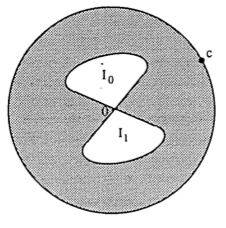
\includegraphics{lobes1.png}}
\newthought{The above characterization} of Julia sets provides a method of construction based on 
a given function $Q_c$. The key idea is that inverting the quadratic function and 
applying the Boundary Mapping Principle gives us a system of nested ``figure-eight''
lobes within lobes.
\marginnote{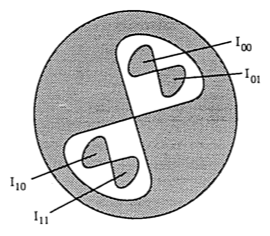
\includegraphics{lobes2.png}}

More specifically, begin with a disk of radius $|c|$ centered at the origin. We can take reverse-iterations of $Q_c$ by subtracting $c$ from all points, then taking their square root. The shape this process yields is one similar to the picture on the left. The lemniscate-like shape has two lobes, each of which has a diffeomorphic mapping to its entire 'parent' lobe or disk. 

It is plain to see that we have $2^k$ unique disjoint lobes at the $k^{\text{th}}$ iteration. We can precisely 
identify a unique lobe via the following. Define 
\begin{align*}
I_{s_0s_1\ldots s_n} = \{z\in D \; | \;  z \in I_{s_0}, Q_c(z) \in I_{s_1}, \ldots, Q_c^{\circ n}(z) \in I_{s_n}\}
\end{align*}
Just as we did with with the quadratic map in the real interval $[0,1]$, we can identify a unique string on two
symbols with each node. When those strings are of infinite length we have that, 
for any $z \in \bigcap_{n\ge 0} I_{s_0s_1\ldots s_n}$, $Q_c^{\circ k} (z) \in D$ for all $k$. Hence, $z \in K_c$. 

This brings us to a more in-depth discussion of $K_c$.
Define a \textsl{component} of $K_c$ is defined as an infinite 
intersection of lemniscates and their lobes. Two components are necessarily disjoint.

Conversely, any $z \in K_c$ must lie in exactly one of these components, since any infinite string of $1$s and $0$
maps to any $z$ by $S(z) = s_0s_1\ldots s_n$ provided $z\in \bigcap_{n\ge 0} I_{s_0s_1 \ldots s_n}$.

Similar arguments to those we used for the Cantor set yield that [1] this correspondence is continuous and [2] that each of these infinite intersections is exactly a single point in the complex plane. The mechanics behind this exceed the scope of this lecture (and class), so we will not include them here.


We additionally give the following remarks without proof, since they would go beyond the scope of our talk. 
They are interesting facts that are good to know, however.


\begin{rmk}
$Q_c$ is supersensitive on $J_c$. Roughly, (as handwavy as Devaney), this is because we can, for any point $z \in I_{s_0s_1\ldots s_k}$, find a small enough disk $D_{\epsilon}$ that contains $z$ such that for an arbitrarily large $k$ we have $Q_c^{\circ k}(D_{\epsilon}) = D$ ($D = B(|c|,0)$). Further iterations of $Q_c$ will eventually diffeomorphically map that disk to 
all of $\mathbb{C}$ (except for at most 1 point).
\end{rmk}


\begin{rmk}
Since $K_c$ is a Cantor set (each component of $K_c$ is a point) when $|c| > 2$, the Julia and filled Julia sets are identical ($K_c = J_c$).
\end{rmk}


\begin{rmk}
When $|c| > 2$, the orbit of 0 tends to $\infty$. This was important in the talk given by the group that
covered the Mandelbrot set.
\end{rmk}



\newthought{In our talk,} we also showed some good images of various Julia sets. Here are some of the links we used.

This website gives an amazing visual intuition for the process we just described
\begin{itemize}
{\color{DeepSkyBlue4}
	\item \href{http://acko.net/blog/how-to-fold-a-julia-fractal/}{Acko - How to Fold a Julia Fractal}
	\item \href{http://demonstrations.wolfram.com/JuliaSetsAndTheMandelbrotSet/}{A demo of Julia-Mandelbrot correspondence}
	\item \href{http://www.juliasets.dk/UFP.htm}{Some pictures of generalized Julia sets}
}
\end{itemize}

Finally, in the following two sections, we discuss two algorithms for generating some of the pictures
you can find on these websites. 

% Section 16.4
\section{16.4 -- Computing the Filled Julia Set}\label{sec:problem-1}


\begin{algorithm}[H]
  \SetKwFunction{KwPaint}{paintBlack} 
  \SetKwFunction{KwMax}{max} 
  \DontPrintSemicolon
  \LinesNumbered

\KwIn{grid, a list of evenly-spaced complex numbers in a rectangular region of the complex plane. MaxIter, the number of iterations to perform}

\For{$j  \leftarrow 1$ to $MaxIter$}{
	\For{$z$ in $grid$}{
		$z \leftarrow Q_c(z)$ \;
	}
}
		\tcp*{Shade all points which didn't escape}
\For{$z$ in $grid$} {
	\If{$|z| \le max(|c|,2)$}{
		\KwPaint{z}\;
	}
}
\caption{Algorithm to plot $K_c$ }
\end{algorithm}







% Section 16.6
\section{16.6 -- Computing the Julia Set Another Way}\label{sec:problem-1}

If we are only interested in the Julia set itself, and not the filled Julia set,
there is an even faster algorithm we can use.
Recall that $Q_c$ is supersensitive on $J_c$. 
This means that any neighborhood $B$ of some point $z\in J_c$ has
the property that 
$\bigcup_{n=0}^\infty Q_0^{\circ n} (B) = \mathbb{C} \setminus \{p\}$ for at most one point $p$.

\vspace{.4cm}

Hence, upersensitive points serve as `attractors' for the backward iteration of $Q_c$, 
in the sense that for each supersensitive point, all of $\mathbb{C}$ except at most one point
must come arbitrarily close to it on reverse iteration. 

\vspace{1cm}
\begin{algorithm}[H]
  \SetKwFunction{KwRand}{randomBit} 
  \SetKwFunction{KwPaint}{paintBlack} 
  \SetKwFunction{KwRandC}{randomComplexNumber} 
  \DontPrintSemicolon
  \LinesNumbered
\KwIn{MaxIter, the maximum number of iterations to perform}


$z \leftarrow $ \KwRandC{}\;
\For{$j  \leftarrow 1$ to \ArgSty{MaxIter}}{
	$binaryRand \leftarrow $ \KwRand{} \;

		\tcp*{Pick a random backwards iteration}	
	\If{$binaryRand = 0$}{
		$z \leftarrow \sqrt{(z-c)}$\;
	} \Else{
		$z \leftarrow -\sqrt{(z-c)}$\;
	}

		\tcp*{Don't plot stray points}
	\If{$j > 100$}{
		\KwPaint{z}   \;
	}


}

\caption{Algorithm to plot $J_c$ }

\end{algorithm}




\end{document}
